\section{Experimental Setup}
\label{sec:exp}

\subsection{Dataset}

ETTh1 is the hourly subset of the Electricity Transformer Temperature dataset introduced with Informer~\cite{informer} and distributed through the ETDataset repository~\cite{ettdata} and the Time-Series-Library~\cite{tslib_code}. The file covers 1 July 2016 to 26 June 2018 (17,420 hourly records) from one power transformer in China. It has seven variables: six load features (high, middle and low useful and useless load: HUFL, HULL, MUFL, MULL, LUFL, LULL) and the oil temperature OT. We found no missing values, no duplicate timestamps and no gaps in the hourly spacing. The load features contain negative values and large excursions (HUFL ranges from $-22.7$ to $23.6$), which we keep because they are part of the recorded signal. The data contain no personal information.

Following the standard protocol, the first 12 months form the training set, the next four months the validation set and the following four months the test set; the remaining 3,020 hours are not used. Table~\ref{tab:split} gives the periods and window counts, and Fig.~\ref{fig:dataset} shows two of the variables with the split. The test period falls in winter. Its mean oil temperature is 4.85 against 17.13 in the training year, and the standard deviation of HUFL is 7.66 against 5.81, so even the clean test set is shifted relative to training. Because windows are cut with stride 1, neighbouring samples overlap and are not independent.

\begin{table}[!t]
\centering
\caption{Chronological Split of ETTh1}
\label{tab:split}
\footnotesize
\colfit{%
\begin{tabular}{@{}llr@{}}
\toprule
Split & Period (hourly records) & Windows ($L{=}336$, $H{=}96$) \\
\midrule
Train & 2016-07-01 to 2017-06-25 (8,640) & 8,209 \\
Validation & 2017-06-26 to 2017-10-23 (2,880) & 2,785 \\
Test & 2017-10-24 to 2018-02-20 (2,880) & 2,785 \\
\bottomrule
\end{tabular}}
\end{table}

\begin{figure*}[!t]
\centering
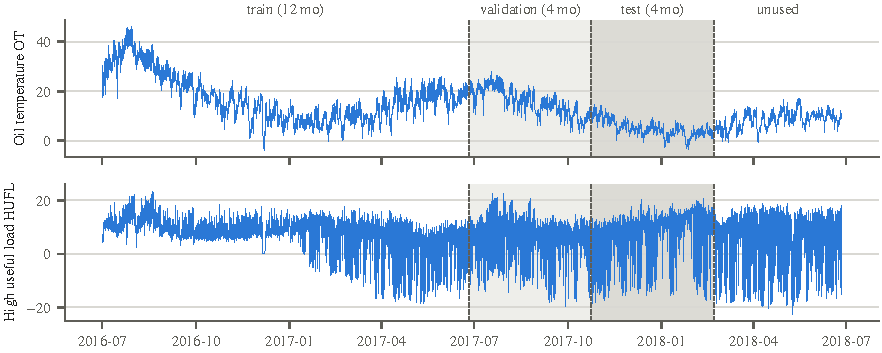
\includegraphics[width=\figwidth]{fig_dataset.pdf}
\caption{Two ETTh1 variables over the full recording with the chronological split. The shaded regions are the validation and test periods; the last 3,020 hours are not used.}
\label{fig:dataset}
\end{figure*}

\subsection{Test Conditions}

Each model is evaluated on 22 versions of the 2,785 test windows (Table~\ref{tab:settings}): the clean inputs, four severity levels for each of the five corruption families, and the mixed setting. Only the input windows are corrupted; the target is the clean future in every case. The mixed setting combines all four training families but at a fixed combination never seen during training.

\begin{table}[!t]
\centering
\caption{The 22 Test Conditions}
\label{tab:settings}
\footnotesize
\renewcommand{\arraystretch}{1.12}
\colfit{%
\begin{tabular}{@{}p{0.28\linewidth}p{0.36\linewidth}p{0.24\linewidth}@{}}
\toprule
Family & Parameters & Levels \\
\midrule
Clean & none & 1 \\
Missing (point) & fraction $p$ of values set to 0 & $p\in\{1,5,10,15\}\%$ \\
Missing (16-stretch) & stretches of 16 zeros, coverage $\approx p$ & $p\in\{1,5,10,15\}\%$ \\
Noise & $+\mathcal{N}(0,1)$ on fraction $p$ & $p\in\{1,5,10,15\}\%$ \\
Anomaly (spike) & $\pm\,\mathcal{U}(3,5)$ on fraction $p$ & $p\in\{1,5,10,15\}\%$ \\
Shift & $k$ segments of 33 steps, $\alpha\!\sim\!\mathcal{U}(0.5,2)$, $\beta\!\sim\!\mathcal{U}(-2,2)$ & $k\in\{1,3,5,10\}$ \\
Mixed & shift $k{=}1$ + noise, spike, missing at 5\% each & 1 \\
\bottomrule
\end{tabular}}
\end{table}

\subsection{Metrics}

We report the mean squared error and mean absolute error on the scaled data,
\begin{equation}
\begin{gathered}
\mathrm{MSE}=\frac{1}{|\mathcal{T}|HC}\sum_{\mathcal{T}}\sum_{i=1}^{H}\sum_{c=1}^{C}(\hat{y}_{i,c}-y_{i,c})^2,\\
\mathrm{MAE}=\frac{1}{|\mathcal{T}|HC}\sum_{\mathcal{T}}\sum_{i=1}^{H}\sum_{c=1}^{C}|\hat{y}_{i,c}-y_{i,c}|,
\end{gathered}
\label{eq:metrics}
\end{equation}
where $\mathcal{T}$ is the set of test windows; lower is better for both. Scaled units make the numbers comparable with published ETTh1 results. Results are aggregated by family (mean over the four levels) and as the mean over all 21 corrupted conditions. Relative change against a reference variant is $\Delta=100\,(\mathrm{MSE}_{v}/\mathrm{MSE}_{\mathrm{ref}}-1)\%$, computed from seed-averaged values, so negative values mean improvement. Gate behaviour is measured as the mean gate weight over corrupted and over clean patches.

\subsection{Statistical Treatment}

Each variant was trained with two seeds (2021 and 2022). We report means with the sample standard deviation over the two seeds, the per-seed values for the headline numbers, and a paired comparison of each variant with A1 in each seed. Two seeds and overlapping test windows do not support formal significance tests or confidence intervals, so we do not report any; the standard deviations should be read as indicating the spread between two runs, nothing more.

\subsection{Baselines}

The baseline is our PatchTST re-implementation (A0). No other published method was re-run under this protocol, so the paper makes no claim about RA-PatchTST relative to DLinear, iTransformer, SEER, TFPS, APT or any other model.
